\documentclass[10pt,twocolumn]{article}
\usepackage[english]{babel} 
\usepackage[T1]{fontenc}
\usepackage{url,color} % Citation numbers being automatically sorted and properly "compressed/ranged". 


\usepackage{graphics,amsfonts}
\usepackage[pdftex]{graphicx}
\usepackage[cmex10]{amsmath}
% Also, note that the amsmath package sets \interdisplaylinepenalty to 10000
% thus preventing page breaks from occurring within multiline equations. Use:
 \interdisplaylinepenalty=2500
% after loading amsmath to restore such page breaks as IEEEtran.cls normally does.
\usepackage[utf8]{inputenc}
\usepackage{csquotes}
%% Useful packages for creation of two-column and more complex figures
% Compact lists
\usepackage{enumitem}

\usepackage{array}
% http://www.ctan.org/tex-archive/macros/latex/required/tools/
\usepackage{mdwmath}
\usepackage{mdwtab}
%mdwtab.sty	-- A complete ground-up rewrite of LaTeX's `tabular' and  `array' environments.  Has lots of advantages over
%		   the standard version, and over the version in `array.sty'.
% *** SUBFIGURE PACKAGES ***
\usepackage[tight,footnotesize]{subfigure}

\usepackage[top=1.5cm, bottom=2cm, right=1.6cm,left=1.6cm]{geometry}
\usepackage{indentfirst}

\usepackage{times}
\usepackage[backend=biber, style=alphabetic, sorting=ynt]{biblatex}
\addbibresource{bibliografia.bib}
%\usepackage[active]{srcltx}
\graphicspath{{./figure/}}

\setlength\parindent{0pt}
\linespread{1}

\def\C#1{\mathcal{#1}}

\renewcommand{\phi}{\varphi}

% FORMATTING
\newcommand{\ie}{i.e.,\,}
\newcommand{\eg}{e.g.,\,}
\newcommand{\columnbreak}{\vfill\eject} % Column break

% REFERENCES
\newcommand{\Fig}[1]{Fig.~\ref{#1}}
\newcommand{\eq}[1]{(\ref{#1})}
\newcommand{\Tab}[1]{Tab.~\ref{#1}}
\newcommand{\Sec}[1]{Sez.~\ref{#1}}


\begin{document}
\title{Robotica autonoma - Progetto finale \\``Handwriting''}
\author{Alberto Cenzato}
\maketitle

\section{Introduzione}
In questo progetto si è cercato di far riprodurre ad un braccio robotico il
movimento di scrittura compiuto da un operatore umano. Nel ciclo di percezione,
ragionamento e azione compiuto dal robot si è posta particolare attenzione alla
parte di percezione dell'azione di scrittura. La prima parte del lavoro è
consistita nella costruzione di un piccolo dataset video. Successivamente è
stato necessario integrare all'interno del progetto ROS due librerie: OpenPose
per l'identificazione della mano dell'operatore all'interno del piano immagine e
AprilTag per avere un sistema di riferimento relativo al piano di scrittura.
Infine, dopo aver estratto dal video 3D la traiettoria della mano, questa è
stata pulita e filtrata per rimovere eventuali outliers.

\begin{figure}[h]
  \centering	
  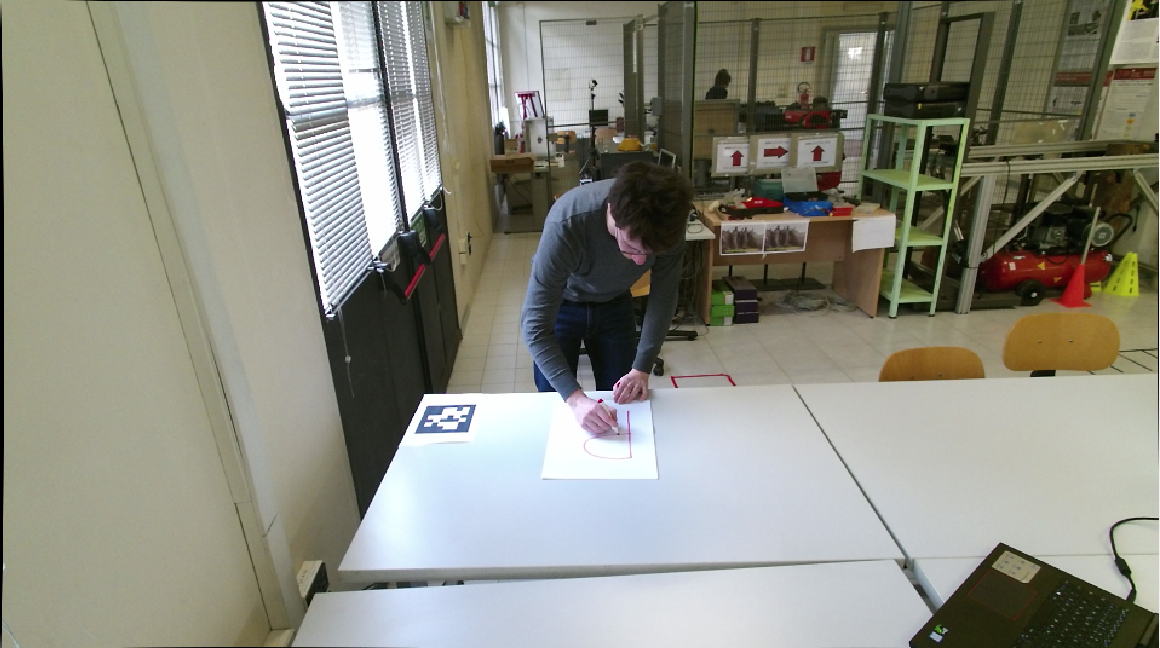
\includegraphics[width=\linewidth]{immagini/setup.png}
  \caption{Un frame di esempio preso da uno dei video.}
  \label{f:setup}
\end{figure}


\section{Setup}
Non avendo a disposizione un dataset per testare il software sono stati
registrati con una Kinect2 $9$ video in cui viene ripreso integralmente
l'operatore mentre scrive una lettera \textbf{P} su un foglio A3 variando di
volta in volta l'orientazione del foglio rispetto alla camera. I video
comprendono non solo l'azione di scrittura, ma anche i momenti precedenti e
successivi ad essa. Sul piano di scrittua è stato posto un tag AprilTag come
origine del sistema di riferimento per la mano rispetto al tavolo. I video sono
stati registrati come \verb|.bag| per poter essere comodamente riprodotti con
\verb|rosbag|.


\section{Algoritmi}
  \subsection{OpenPose}
  OpenPose\footnote{https://github.com/CMU-Perceptual-Computing-Lab/openpose} è
  una libreria C++ sviluppata dal Perceptual Computing Lab della Carnegie Mellon
  University \cite{cao2017realtime}. È in grado di identificare con precisione
  la posizione nel piano immagine degli arti di una persona a partire da una
  singola immagine RGB processando diversi frame al secondo. \\ 
  OpenPose usa una \textit{convolutional neural network} suddivisa in due rami:
  un ramo della rete si occupa di calcolare una confidence map per ogni parte
  del corpo producendo $J$ matrici $S^j \in \mathbb{R}^{w \times h}$ dove $J$ è
  il numero di parti del corpo mentre $w$ e $h$ sono rispettivamentne larghezza
  e altezza dell'immagine in input; il secondo ramo della rete si occupa di
  predirre in una matrice $L \in \mathbb{R}^{w \times h \times 2}$ i
  \textit{part affinity fields} ossia il grado di confidenza che due parti siano
  collegate da un arto. L'immagine, prima di essere data in input alla rete,
  viene processata dai primi 10 layer di VGG-19 \cite{simo2015verydeepconv} (già
  allenata separatamente) in modo da fornire ai due rami della rete delle
  features di alto livello. Ogni ramo della rete migliora iterativamente la
  predizione: alla fine di ogni iterazione $S^i$, $L^i$ e la feature map $F$
  estratta con VGG-19 vengono concatenate per formare l'input per
  l'iterazione successiva (si veda \Fig{f:openpose_cnn}). Come \textit{loss
  function} viene usata la somma del MSE dell'output di ogni iterazione. 
  
  \begin{figure}[h]
    \centering
    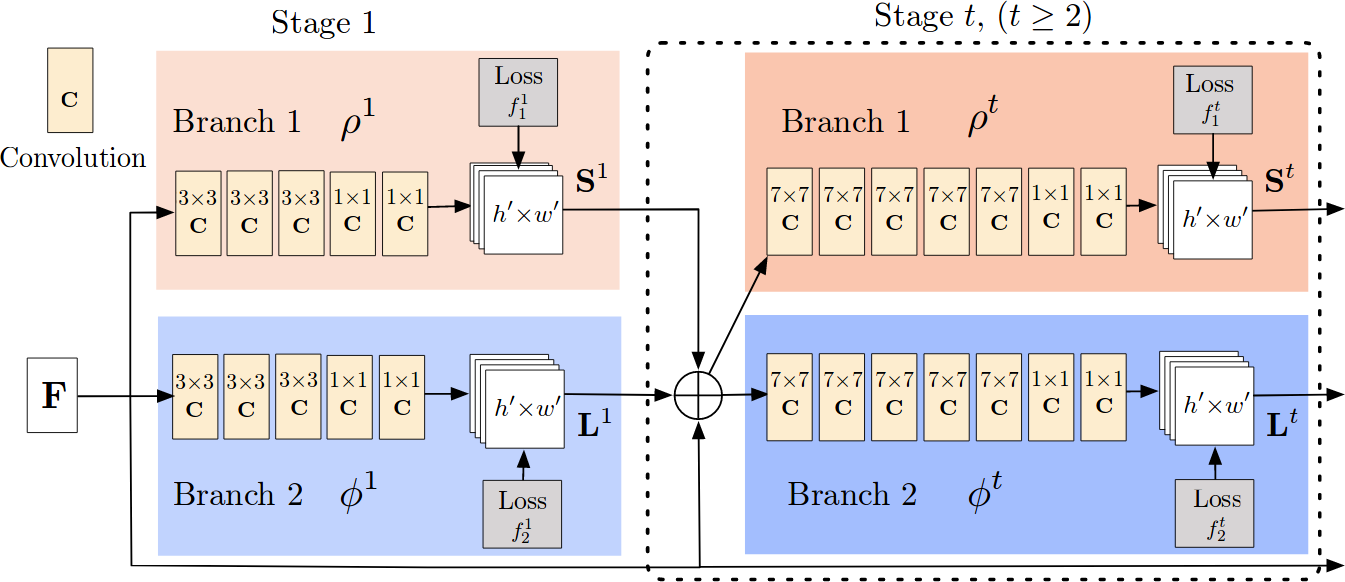
\includegraphics[width=\linewidth]{immagini/openpose-cnn.png}
    \caption{Architettura dei primi due stadi della rete di OpenPose.}
    \label{f:openpose_cnn}
  \end{figure}

  Individuate le parti del corpo è necessario associarle tra loro a coppie per
  identificare gli arti. Questo problema di ottimizzazione combinatoria è
  NP-hard, di conseguenza OpenPose sfrutta una strategia greedy per risolvere
  una versione rilassata del problema con l'aiuto dei \textit{part affinity
  fields} precedentemente calcolati. Ogni matrice $L$ rappresenta un campo
  vettoriale in due dimensioni che codifica la posizione e l'orientazione di
  ogni arto. Per una coppia di parti del corpo $d_{j_1}$ e $d_{j_2}$
  la confidenza con la quale fanno parte dello stesso arto è l'integrale di
  linea:
  
  \newcommand{\vardist}{d_{j_2} - d_{j_1}}
  \newcommand{\varinterpol}{(1 - u)d_{j_1} + ud_{j_2}}
  \begin{equation}
    E = \int_{u=0}^{u=1} L_c\big(\varinterpol\big) \cdot \frac{\vardist}{||\vardist||_2} du
  \end{equation}
  
  Usando i valori di $E$ così calcolati viene costruito un grafo pesato dove i
  nodi sono le parti del corpo. Per semplificare il problema altrimenti
  intrattabile il grafo non è completamente connesso: ogni $i$-esima parte del
  corpo della persona $j_1$, viene connessa con le parti del corpo ad essa
  vicina di ogni altra persona; ad esempio ogni gomito sarà connesso ad ogni
  polso e ad ogni spalla, ma non al ginocchio. Dal risultante grafo si cerca i
  sottografi di peso massimo. Questi corrisponderanno alle persone presenti
  nell'immagine.

  \subsection{AprilTag}
  AprilTag \cite{olson2011tags} è un sistema di localizzazione visiva che
  permette l'dentificazione della posizione in tutti e 6 i gradi di libertà a
  partire da una singola immagine usando dei tag composti da quadrati bianchi e
  neri (si veda \Fig{f:apriltag} per un esempio). 
  
  \begin{figure}[h]
    \centering
    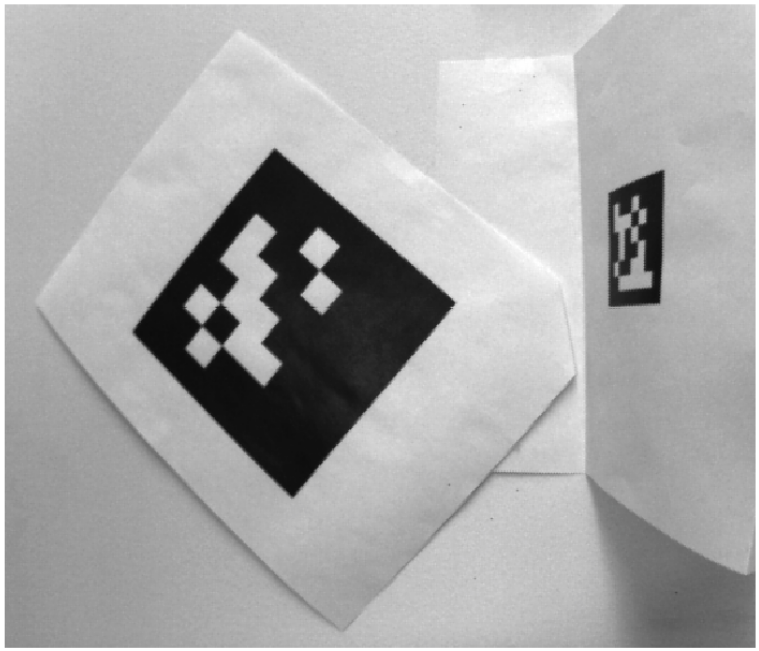
\includegraphics[width=\linewidth]{immagini/apriltag.png}
    \caption{Due esempi di tag.}
    \label{f:apriltag}
  \end{figure}
  
  Il sistema è composto da due parti: un detector e un decoder. Il detector
  cerca di identificare quadrilateri con l'interno più scuro rispetto
  all'esterno. Come prima cosa viene calcolata la direzione del gradiente e la
  sua intensità per ogni pixel; successivamente vengono raggruppati insieme i
  pixel con direzione e intensità del gradiente simili costrudendo un grafo
  formato da un nodo per ogni pixel. Il nodo per il pixel $p_{i,j}$ è connesso
  ai nodi dei pixel adiacenti a $p_{i,j}$; ogni arco ha un peso pari alla
  differenza di direzione del gradiente tra i due pixel. Poi si procede a
  raggruppare i pixel; per ogni arco si uniscono i due gruppi a cui appartengono
  i pixel da esso connessi se sono soddisfate le seguenti condizioni:
  
  \begin{eqnarray}
    D(n \cup m) & \leq & min\{D(n), D(m)\} + \frac{K_D}{|n \cup m|} \\
    M(n \cup m) & \leq & min\{M(n), M(m)\} + \frac{K_M}{|n \cup m|} 
  \end{eqnarray}

  dove $D()$ indica la differenza tra il minimo e il massimo valore della
  direzione del gradiente, $M()$ la differenza di minima e massima intensità del
  gradiente e $n$ e $m$ sono i due gruppi candidati per l'unione. Quindi due
  gruppi sono uniti se la loro unione è più o meno uniforme quanto i due gruppi
  presi singolarmente. Una volta individuate le componenti connesse viene
  effettuato un fit ai minimi quadrati per identificare i segmenti presenti
  nell'immagine. Infine i segmenti sono raggruppati a gruppi di 4 per formare i
  quadrilateri. \\
  Posizione e orientazione del tag vengono ricostruiti calcolando innanzitutto
  l'omografia che proietta i punti 2D dal sistema di coordinate del tag in
  quello dell'immagine; dopodiché, note l'omografia $H$ e la matrice intrinseca
  della camera $P$ viene calcolata la matrice estrinseca $E$:

  \begin{eqnarray*}
    H      & = & sPE \\
           & \downarrow & \\
    h_{00} & = & sR_{00}f_x \\
    h_{01} & = & sR_{01}f_x \\
    h_{02} & = & sT_xf_x \\
           & \vdots &
  \end{eqnarray*}

  dove $s$ è il fattore di scala. \\
  Il tag contiene anche un payload, dando la possibilità di distinguere più tag
  in movimento all'interno di una sequenza di immagini. Tuttavia, avendo in
  questo progetto un solo tag, questa funzionalità non è stata utilizzata.

  \subsection{Estrazione della traiettoria}
  \label{sec:alg_traiettoria}
  Integrando le capacità di OpenPose e AprilTag in un unico software è stato
  possibile estrarre dal video RGBD, composto da immagini a colori $I_{RGB}$ e
  immagini di profondità $I_{D}$, la traiettoria compiuta dalla mano. Usando i
  frame $I_{RGB}$ sono state individuate le posizioni dei giunti della mano nel
  piano immagine attraverso OpenPose. Il centro della mano è stato individuato
  come il centroide $m^{img}$ di questi punti. La posizione della mano rispetto
  all'asse $z$ nel sistema di riferimento della camera $m_z^{cam}$ è data dalla
  media di $z$ in un piccolo intorno di $m^{img}$. Per spostare le coordinate di
  $m^{img}$ nel sistema di riferimento della camera si sfrutta la matrice
  intrinseca della camera:
  
  \begin{eqnarray}
    m_x^{cam} & = & \frac{m_z^{cam} (m_x^{img} - c_x)}{f_x} \\
    m_y^{cam} & = & \frac{m_z^{cam} (m_y^{img} - c_y)}{f_y} \\
    m_z^{cam} & = & m_z^{cam}
  \end{eqnarray}

  I punti $m^{cam}$ sono trasformati nel sistema di riferimento del tag posto
  sul tavolo ottenendo $m^{tag} \in T^{tag}$ dove $T^{tag}$ è la traiettoria
  completa (se ne può vedere un esmpio in \Fig{f:trajectory}). I punti $m^{tag}$
  vengono poi filtrati secondo tre criteri:
  \begin{itemize}
    \item se $|m_z^{tag}| > th$ dove $th$ è una soglia fissata, cioè se il punto è
    troppo distante dal piano di scrittura, allora il punto viene scartato;
    \item se la velocità della mano in un punto $m^{tag}$ è più alta del doppio della
    velocità media degli altri punti, allora quel punto $m^{tag}$ viene scartato;
    \item dato il centro della traiettoria 
      $$c^{tag} = \frac{1}{|T^{tag}|} \sum_{m^{tag} \in T^{tag}} m^{tag}$$ 
      e la distanza media dei punti da questo 
      $$\overline{d} = \frac{1}{|T^{tag}|} \sum_{m^{tag} \in T^{tag}}||m^{tag}-c^{tag}||_2$$
      vengono eliminati tutti i punti
      $$m^{tag} \in T^{tag} \colon\ ||m^{tag} - c^{tag}||_2 >  2\overline{d}$$
  \end{itemize}

  Con queste tre semplici regole si ottengono degli ottimi risultati, come si
  può vedere in \Fig{f:final_trajectory}, senza la necessità di identificare
  quel è stato scritto.

  \begin{figure}[h]
    \centering
    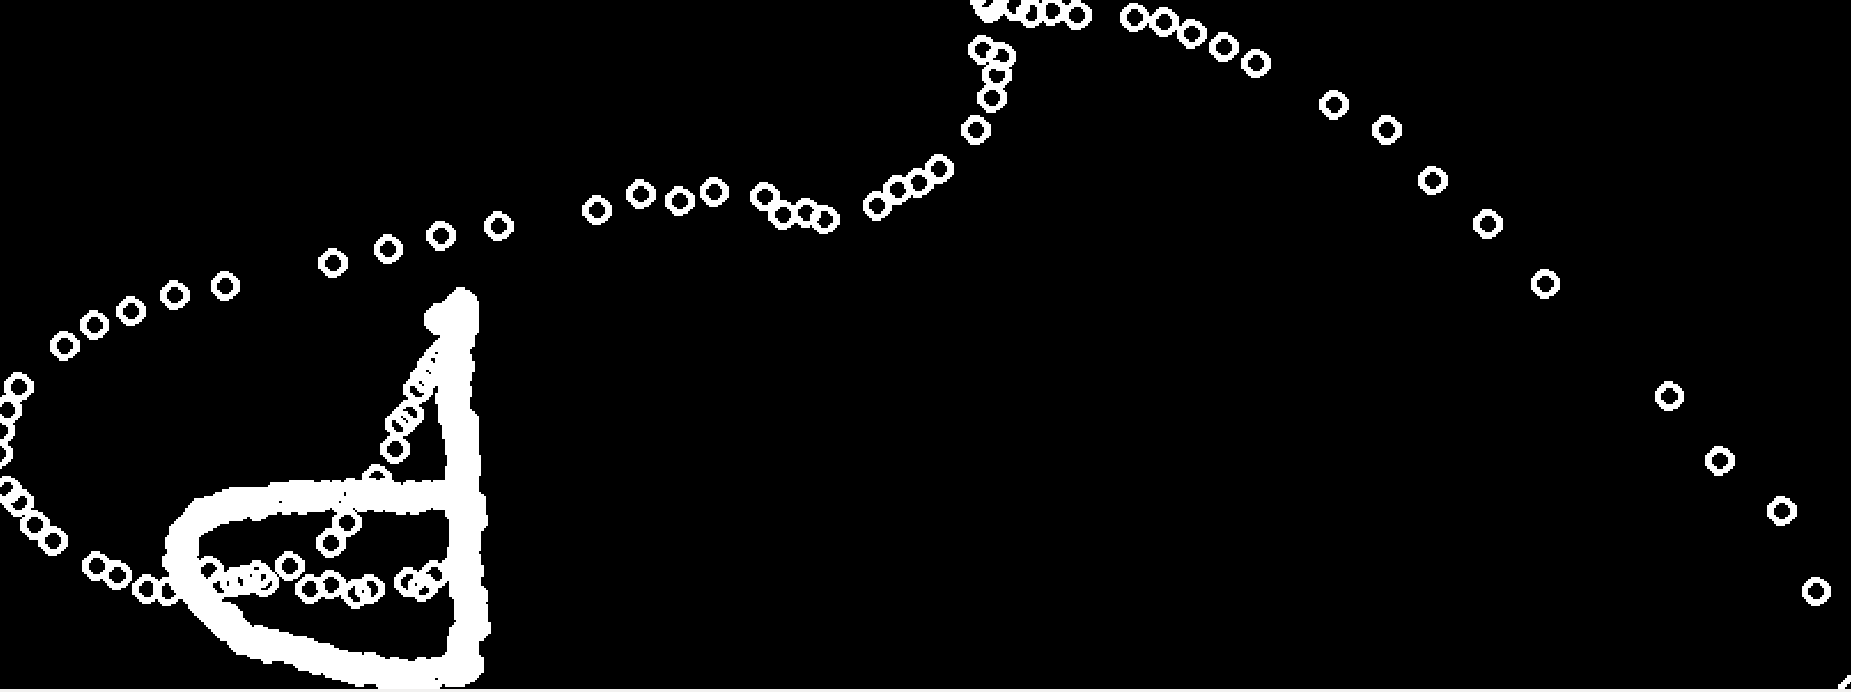
\includegraphics[width=\linewidth]{immagini/trajectory.png}
    \caption{La traiettoria estratta dal video RGBD.}
    \label{f:trajectory}
  \end{figure}


\section{Implementazione}
L'implementazione, inizialmente prevista come una semplice composizione di
pezzi, si è rivelata più complessa del previsto. Il progetto finale si compone
di tre nodi ROS: uno che riceve i frame RGB e li processa con OpenPose, uno che
estrae le \verb|tf| ROS attraverso AprilTag e infine uno che raccolglie i punti della
traiettoria in un'unica lista, li porta nel sistema di riferimento del tag,
filtra la traiettoria e la pubblica.

  \subsection{Nodo openpose\_ros}
  \label{sec:openpose_ros}
  L'implementazione C++ di OpenPose viene distribuita opensource, di conseguenza
  sono disponibili diversi fork e wrapper che includono OpenPose in un nodo ROS.
  Purtroppo è stato difficile trovare un wrapper funzionante; dopo aver provato
  senza successo tre implementazioni tra le più utilizzate è emerso chiaramente
  un problema di versionamento del software: molti di quei wrapper erano stati
  scritti per una versione specifica di OpenPose, il quale nel frattempo era
  stato aggiornato e aveva cambiato più volte le sue API; nessuno dei wrapper
  però indicava per quale verisone di OpenPose fosse stato scritto. \\
  La soluzione è stata quella di scegliere il wrapper più promettente,
  effettuarne un fork e sistemare i bug affinché funzionasse con l'ultima
  versione di OpenPose allora disponibile. Sono anche stati apportati alcuni
  miglioramenti minori aggiungendo agli header dei messaggi pubblicati da
  \verb|openpose_ros| il timestamp (\verb|stamp|) e il numero sequenziale
  (\verb|seq|) del frame che è stato processato per generare il messaggio. In
  questo modo è possibile associare più facilmente la posa di un soggetto con il
  frame da cui è stata ricavata, funzionalità utile nel caso un cui più nodi
  abbiano la necessità di processare la stessa immagine. \\
  Anche questa ennesima versione è disponibile su
  GitHub\footnote{\url{https://github.com/AlbertoCenzato/openpose_ros}}
  includendo, tuttavia, a differenza degli altri, un submodule git contenente il
  commit di OpenPose per cui è stata creata in modo da evitare ogni ambiguità e
  incompatibilità tra versioni. 

  \begin{figure}[h]
    \centering
    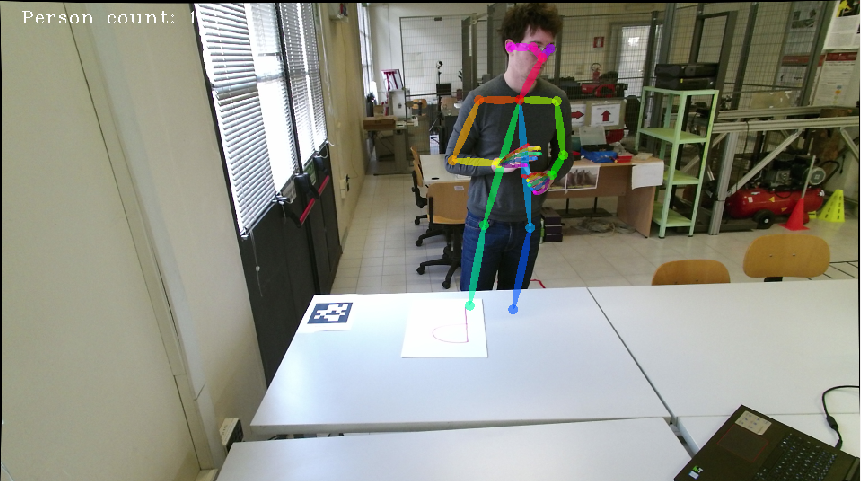
\includegraphics[width=\linewidth]{immagini/openpose_person_detection.png}
    \caption{Identificazione della posizione degli arti con openpose}
    \label{f:person_detection}
  \end{figure}

  \subsection{Nodo apriltags\_ros}
  La libreria AprilTag era inizialmente stata inserita all'interno del nodo
  \verb|handwriting|. L'implementazione C di AprilTag è stata parzialmente
  modificata per avere un'interfaccia ad oggetti e quindi essere più facilmente
  integrabile con il resto del progetto in C++. La scelta di avere AprilTag
  all'interno del nodo handwriting è stata fatta per minimizzare il numero di
  nodi ROS e il passaggio di messaggi. Tuttavia questa implementazione è stata
  successivamente scartata in favore di un nodo AprilTag a sè stante. Questa
  scelta è stata dettata dalla decisione di mantenere il progetto il più
  modulare possibile per seplificare la manutenzione, l'integrazione con altri
  nodi ROS ed evenutali modifiche future a scapito dell'effcienza; è infatti
  necessario un processo attivo in più.

  \subsection{Nodo handwriting}
  Il nodo \verb|handwriting| si occupa di mettere insieme le informazioni
  ricavate con \verb|openpose_ros| e \verb|apriltags_ros|. Dopo una fase di
  inizializzazione in cui recupera la matrice intrinseca della camera pubblicata
  dalla kinect e le \verb|tf| pubblicate da \verb|apriltags_ros| il nodo
  \verb|handwriting| inizia il ciclo di raccolta dei punti della traiettoria. Il
  nodo riceve l'immagine RGB, l'immagine di profondità e le posizioni dei giunti
  del corpo. Dopo aver individuato nel frame $t$ la posizione della mano nel
  sistema di riferimento della camera $p^{cam}_t \in \mathbb{R}^3$ come
  descritto in \Sec{sec:alg_traiettoria}, lo aggiunge alla lista che contiene
  $p^{cam}_\tau$ con $\tau < t$. Il ciclo di raccolta dei punti viene interrotto
  dopo che il nodo non ha ricevuto alcun frame per almeno $5$ secondi. Infine i
  punti vengono trasformati nel sistema di riferimento del tag e vengono rimossi
  quelli che non appartengono alla traiettoria di scrittura della lettera.

  \begin{figure}[h]
    \centering
    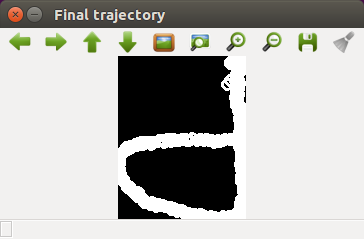
\includegraphics[width=\linewidth]{immagini/final_trajectory.png}
    \caption{La traiettoria filtrata contenente solo i punti appartenenti alla lettera.}
    \label{f:final_trajectory}
  \end{figure}

  L'associazione tra i punti della mano nell'immagine RGB e i loro corrispettivi
  nell'immagine di profondità ha richiesto la sincronizzazione dei messaggi
  pubblicati da \verb|openpose_ros| con la relativa immagine di profondità.
  Fortuantamente ROS possiede già la classe
  \verb|message_filters::TimeSynchronizer| che è pensata proprio a questo scopo;
  non è stato perciò necessario implementare un'ulteriore coda di messaggi per
  la sincronizzazione, ma è bastato modificare leggermente il codice di
  \verb|openpose_ros| (si veda \Sec{sec:openpose_ros}). \\
  Tutta la logica del nodo ad eccezione della pubblicazione finale della
  traiettoria è contenuta nella classe \verb|Handwriting| che è stata scritta in
  modo da fornire un'interfaccia con chiamate sincrone che va a nascondere la
  natura necessariamente asincrona di ROS e dell'estrazione della traiettoria.
  Il nodo, dal suo punto di vista, ottiene le traiettorie complete (nel sistema
  di riferimento della camera e in quello del tag) attraverso una semplice
  chiamata bloccante a \verb|Handwriting::getTrajectories()|. Questo approccio
  non richiede sincronizzazioni, spin o altro e, fornendo la classe come un
  pacchetto completo e autocontenuto, dovrebbe semplificare l'eventuale
  integrazione con altri pezzi di codice.


\section{Considerazioni e sviluppi futuri}
Lo svolgimento del progetto ha richiesto per la maggior parte un lavoro di
documentazione e studio di algoritmi e librerie preesistenti e soprattutto di
integrazione di queste con parti di codice ad hoc. Lo studio delle librerie non
si è limitato alle API esposte, ma anche ad alcuni dettagli interni, dovendo
adattarle alle esigenze del progetto. Dal punto di vista algoritmico non ci sono
state grosse difficoltà nella scrittura del nodo \verb|handwriting| in quanto
non contiene una logica particolarmente complessa. \\
Volendo proseguire e migliorare il lavoro si potrebbe intervenire in almeno due
modi: 
\begin{itemize}
  \item sulle prestazioni
  \item sull'ambito di applicazione
\end{itemize}
Al momento l'estrazione della traiettoria, per essere accurata, non può essere
fatta in tempo reale. OpenPose, che di fatto risulta essere il collo di
bottiglia di tutto il sistema, riesce ad elaborare circa $10$ frame al secondo
su un pc dotato di una buona GPU\footnote{I test sono stati effettuati con una
GeForce GTX 1060}. Una soluzione potrebbe essere quella di modificare
\verb|openpose_ros| affinché campioni il video in input a $10$Hz \textit{prima}
di identificare la posizione degli arti, dovedo però diminuire l'accuratezza
della traiettoria così indentificata. Un approccio del genere andrebbe però
valutato caso per caso a seconda degli ambiti di applicazione e principalmente
dalla velocità di spostamento della mano dell'operatore. \\
Al momento il progetto è pensato per funzionare nei casi in cui si ha una
ripresa quasi integrale dell'operatore. OpenPose infatti non consente di
determinare la posizione dei giunti della mano se la maggior parte del resto del
corpo è al di fuori del campo visivo della camera. Modificare OpenPose in tal
senso permetterebbe non solo di poter applicare il progetto ad un numero
maggiore di possibili scenari, ma anche guadagnare molto nelle prestazioni.
Dovendo analizzare solamente una mano, sarebbe sufficiente una risoluzione anche
di $10$ volte inferiore. Questo significa una rete più piccola che processa meno
dati, riuscendo probabilmente ad ottenere almeno una trentina di frame al
secondo. Ovviamente questo approccio sarebbe molto più oneroso, dovendo
apportare importanti modifiche a OpenPose e richiedendo di effettuare nuovamente
il training della rete.



\printbibliography

\end{document}
